%%%%%%%%%%%%%%%%%%%%%%%%%%%%%%%%%%%%%%%%%%%%%%%%%%%%%%%%%%%%%%%%%%%%%%%%%%%%%%%%%%%%%%%%%%%%%%%%%%%%%%%%%%%%%%%%%%%%%%%%%%%%%%%%%%%%%%%%%%%%%%%%%%%%%%%%%%%
% This is just an example/guide for you to refer to when producing your supplementary material for your Frontiers article.                                 %
%%%%%%%%%%%%%%%%%%%%%%%%%%%%%%%%%%%%%%%%%%%%%%%%%%%%%%%%%%%%%%%%%%%%%%%%%%%%%%%%%%%%%%%%%%%%%%%%%%%%%%%%%%%%%%%%%%%%%%%%%%%%%%%%%%%%%%%%%%%%%%%%%%%%%%%%%%%

%%% Version 2.5 Generated 2018/06/15 %%%
%%% You will need to have the following packages installed: datetime, fmtcount, etoolbox, fcprefix, which are normally inlcuded in WinEdt. %%%
%%% In http://www.ctan.org/ you can find the packages and how to install them, if necessary. %%%
%%%  NB logo1.jpg is required in the path in order to correctly compile front page header %%%

\documentclass[utf8]{frontiers_suppmat} % for all articles
\usepackage{url,hyperref,lineno,microtype}
\usepackage[onehalfspacing]{setspace}

\setcitestyle{square} % for Physics and Applied Mathematics and Statistics articles
\usepackage{url,hyperref,lineno,microtype,subcaption}
\usepackage[onehalfspacing]{setspace}
\linenumbers
\usepackage{booktabs}
\usepackage{multirow}
\usepackage{siunitx}
\usepackage{tikz}
\usetikzlibrary{positioning}
\usepackage{amsmath}
\usepackage{amssymb, amsfonts}
\usepackage{blkarray}
\usepackage{bigstrut}
\usepackage{multicol}
\usepackage{float}
\usepackage{lscape} 
\usepackage{mathtools,amssymb}                % <---
\usepackage{booktabs, makecell}
\usepackage{array}
\usepackage{algorithm,algorithmic}
\usepackage{bm}



% ----- GREG ADDED THIS TO CREATE CUSTOM COUNTERS FOR THE MIP PROGRAMS




\usepackage{environ}
\newif\ifsolution
\solutiontrue
\newcounter{fakeequation}
\newcounter{fakeeqtmp}
\NewEnviron{MIP.Len}{\setcounter{fakeeqtmp}{\value{equation}}\setcounter{equation}{\value{fakeequation}}%
    \renewcommand\theequation{Edge${}\I_{Len}$}\ifsolution\BODY\fi%
    \setcounter{fakeequation}{\value{equation}}\setcounter{equation}{\value{fakeeqtmp}}\renewcommand\theequation{\arabic{equation}}}
    \NewEnviron{MIP.Unif}{\setcounter{fakeeqtmp}{\value{equation}}\setcounter{equation}{\value{fakeequation}}%
    \renewcommand\theequation{Edge${}\I_{Unif}$}\ifsolution\BODY\fi%
    \setcounter{fakeequation}{\value{equation}}\setcounter{equation}{\value{fakeeqtmp}}\renewcommand\theequation{\arabic{equation}}}
\newcounter{fakeequationLP}
\newcounter{fakeeqtmpLP}    
\NewEnviron{LP.Len}{\setcounter{fakeeqtmpLP}{\value{equation}}\setcounter{equation}{\value{fakeequationLP}}%
    \renewcommand\theequation{Edge${}\NI_{Len}$}\ifsolution\BODY\fi%
    \setcounter{fakeequationLP}{\value{equation}}\setcounter{equation}{\value{fakeeqtmpLP}}\renewcommand\theequation{\arabic{equation}}}
    \NewEnviron{LP.Unif}{\setcounter{fakeeqtmpLP}{\value{equation}}\setcounter{equation}{\value{fakeequationLP}}%
    \renewcommand\theequation{Edge${}\NI_{Unif}$}\ifsolution\BODY\fi%
    \setcounter{fakeequationLP}{\value{equation}}\setcounter{equation}{\value{fakeeqtmpLP}}\renewcommand\theequation{\arabic{equation}}}
    \NewEnviron{LP.Vol}{\setcounter{fakeeqtmpLP}{\value{equation}}\setcounter{equation}{\value{fakeequationLP}}%
    \renewcommand\theequation{Triangle${}\NI_{Unif}$}\ifsolution\BODY\fi%
    \setcounter{fakeequationLP}{\value{equation}}\setcounter{equation}{\value{fakeeqtmpLP}}\renewcommand\theequation{\arabic{equation}}}
    
    \NewEnviron{MIP.Vol}{\setcounter{fakeeqtmpLP}{\value{equation}}\setcounter{equation}{\value{fakeequationLP}}%
    \renewcommand\theequation{Triangle${}\I_{Unif}$}\ifsolution\BODY\fi%
    \setcounter{fakeequationLP}{\value{equation}}\setcounter{equation}{\value{fakeeqtmpLP}}\renewcommand\theequation{\arabic{equation}}}
    \NewEnviron{LP.Area}{\setcounter{fakeeqtmpLP}{\value{equation}}\setcounter{equation}{\value{fakeequationLP}}%
    \renewcommand\theequation{Triangle${}\NI_{Area}$}\ifsolution\BODY\fi%
    \setcounter{fakeequationLP}{\value{equation}}\setcounter{equation}{\value{fakeeqtmpLP}}\renewcommand\theequation{\arabic{equation}}}
    
    \NewEnviron{MIP.Area}{\setcounter{fakeeqtmpLP}{\value{equation}}\setcounter{equation}{\value{fakeequationLP}}%
    \renewcommand\theequation{Triangle${}\I_{Area}$}\ifsolution\BODY\fi%
    \setcounter{fakeequationLP}{\value{equation}}\setcounter{equation}{\value{fakeeqtmpLP}}\renewcommand\theequation{\arabic{equation}}}
    
    

\newcommand{\R}{\mathbb{R}}
\newcommand{\Z}{\mathbb{Z}}
\newcommand{\Q}{\mathbb{Q}}
\newcommand{\field}{\mathbb{F}}
\newcommand{\PH}{\ensuremath{\mathrm{PH}}}
\newcommand{\Chains}{\mathbf{C}}
\newcommand{\p}[0]{\mathbf{p}}
\newcommand{\q}[0]{\mathbf{q}}
\newcommand{\x}[0]{\mathbf{x}}
\newcommand{\y}[0]{\mathbf{y}}
\renewcommand{\u}[0]{\mathbf{u}}
\renewcommand{\v}[0]{\mathbf{v}}
\newcommand{\w}[0]{\mathbf{w}}
\newcommand{\z}[0]{\mathbf{z}}
\newcommand{\Homologies}[0]{\mathbf{H}}
\newcommand{\Boundaries}[0]{\mathbf{B}}
\newcommand{\Simplices}[0]{\mathbf{S}}
\newcommand{\Cycles}[0]{\mathbf{Z}}
\newcommand{\originalrep}{\mathbf{x}^{Orig}}
\newcommand{\optimalrep}{\mathbf{x}}
\newcommand{\orepentry}{x}
\newcommand{\chain}{\mathbf{c}}
\newcommand{\cycle}{{\mathbf z}}
\newcommand{\cycley}{\mathbf{y}}
\newcommand{\cyclea}{\mathbf{a}}
\newcommand{\cycleb}{\mathbf{b}}
\newcommand{\cycleu}{\mathbf{u}}
\newcommand{\cyclev}{\mathbf{v}}
\newcommand{\cyclew}{\mathbf{w}}
\newcommand{\boundingchain}{\mathbf{w}}
\newcommand{\hclass}{h} % arbitrary homology class
\newcommand{\tab}{Table }
\newcommand{\se}{Section }
\newcommand{\fig}{Figure }
\newcommand{\volvec}{\mathbf{v}}
\newcommand{\supp}{\mathrm{supp}}
\newcommand{\eq}{Equation }
\newcommand{\cm}{comment }
\newcommand{\NI}{^{NI}}
\newcommand{\I}{^I}
\newcommand{\unif}{_{Unif}}
\newcommand{\len}{_{Len}}
\newcommand{\area}{_{Area}}
\newcommand{\birth}{\mathrm{Birth}}
\newcommand{\death}{\mathrm{Death}}
\newcommand{\persistencediagram}{\mathrm{Pers}}
\newcommand{\barcode}{\mathrm{Barcode}}
\newcommand{\boundsub}{\partial_2[:,b_i:d_i]}
\newcommand{\boundsubrow}{\partial_2[1:d_i, b_i: d_i]}
\newcommand{\persinterval}{\mathcal{L}}
\newcommand{\closedinterval}{[b_i,d_i]}
\newcommand{\interval}{J}
\newcommand{\loss}{\mathrm{loss}}
\newcommand{\argmin}{\mathrm{argmin}}
\newcommand{\fcyclebasis}{\mathcal{C}}
\newcommand{\setoffilteredcyclebases}{\mathrm{FCB}}
\newcommand{\setofhcyclebases}{\mathrm{HCB}}
\newcommand{\setofpersistenthcyclebases}{\mathrm{PrsHCB}}
\newcommand{\dimss}[1]{^{(#1)}} % dimension superscript (marks the dimension of a simplex)
\newcommand{\pr}{Program }

\newcommand{\spann}{{\mathrm{span}}}

\setlength{\tabcolsep}{1pt}
\renewcommand{\arraystretch}{1.5}

%   HOMOLOGICAL ALGEBRA
\newcommand{\hcyclebasis}{\mathcal B}

%   SIMPLICES
\newcommand{\alldim}{\omega}
\newcommand{\simplex}{\sigma}

%   LINEAR PROGRAMS
\newcommand{\feasibleset}{\mathcal{X}}    
\newcommand{\Edge}{\mathrm{Edge}}
\newcommand{\Tri}{\mathrm{Tri}}

\newcommand{\goodcycleindices}{\mathcal P}
\newcommand{\goodtriangles}{\mathcal Q}
\newcommand{\goodedges}{\mathcal R}
\newcommand{\goodvolmatrix}{\partial_{2}[\mathcal{F}_1, \hat {\mathcal{F}_2}]}

\newcommand{\simplexpairs}{{\mathcal I}}
\newcommand{\bdpairs}{{\mathcal I}}
\newcommand{\deathbasis}{\mathcal D}

\newcommand{\obasis}{Z} % ordered basis
\newcommand{\obasisel}{\mathbf{z}}  % element of an ordered basis

%   FONTS

\newcommand{\cald}{\mathcal D}
\newcommand{\cale}{\mathcal E}
\newcommand{\calf}{\mathcal F} 
\newcommand{\calm}{\mathcal M}
\newcommand{\caln}{\mathcal N}


%   ENVIRONMENTS
\theoremstyle{plain}
\newtheorem{theorem}{Theorem}[section]
\newtheorem{lemma}[theorem]{Lemma}
\newtheorem{corollary}[theorem]{Corollary}
\newtheorem{proposition}[theorem]{Proposition}
\theoremstyle{definition}
\newtheorem{definition}[theorem]{Definition}
\newtheorem{example}[theorem]{Example}
\newtheorem{remark}[theorem]{Remark}

\newcommand{\LZ}[1]{{\textcolor{magenta}{\small {\sf [[LZ: #1]]}}}}
\newcommand{\GHP}[1]{{\textcolor{purple}{\small {\sf [[GHP: #1]]}}}}
\newcommand{\LL}[1]{{\textcolor{blue!50}{\small {\sf [[LL: #1]]}}}}
\newcommand{\CG}[1]{{\textcolor{blue}{\small {\sf [[CG: #1]]}}}}
\newcommand{\CT}[1]{{\textcolor{YellowGreen}{\small {\sf [[CT: #1]]}}}}

% 1-d generator to replace loops
% cycle in homology 
% a generator is a union of simple closed paths



%   GENERATOR COMPUTATION

\newcommand{\low}{\mathrm{low}}
\newcommand{\hatgraph}{{\hat{\Gamma}}}

% reference labels in lists

\makeatletter
\def\namedlabel#1#2{\begingroup
    #2%
    \def\@currentlabel{#2}%
    \phantomsection\label{#1}\endgroup:
}
\makeatother

%   REPLACEMENT REFERENCES

\newcommand{\algtri}{{2}{}} % note: the extra {} corrects a spacing issue
\newcommand{\proedgeloss}{(EDGE LOSS \#){}} % note: the extra {} corrects a spacing issue

% Leave a blank line between paragraphs instead of using \\

\begin{document}
\onecolumn
\firstpage{1}

\title[Supplementary Material]{{\helveticaitalic{Supplementary Material}}}


\maketitle


\section{Review: Standard algorithm to compute persistent homology cycle bases, by matrix decomposition}
\label{sec:computingcyclereps}

The first step in Algorithms 1 and 2 is to compute a persistent homology cycle basis.  The standard method to compute such a basis invokes a so-called $R = DV$ decomposition  of the boundary matrices $\partial_n$ \cite{cohen2006vines}.  Here we  provide a brief review of this process; further details may be found in \cite{cohen2006vines, SMVDualities11}.
  
  To begin, we must place a total order on each set $\Simplices_n(K)$, in ascending order of birth.  This naturally allows us to regard $\partial_n$ as an element of $G^{|\Simplices_{n-1}(K)| \times |\Simplices_{n}(K)|}$.  The \emph{low}  function on a matrix $A \in G^{k \times l}$ is defined by
    \begin{align*}
        \low: \underbrace{\{j : A[:,j] \neq 0 \}}_{\mathrm{domain}(\low)} \to \Z, \quad j \mapsto \max \{i : A[i,j] \neq 0 \}.
    \end{align*}
We say that $A$ is \emph{reduced} if $\low$ is injective.  An $R = DV$ decomposition is a matrix equation where $R$ is reduced and $V$ is invertible and upper triangular.

Suppose that $R_n = \partial_n V_n$ is such a decomposition for each $n$.   Let $\low^n$ be the low function of $R_n$, and let $\Gamma_n = \{(j, \low(j)) : R[:,j] \neq 0\}$ be the graph $\low^n$.  It can then be shown (\cite{cohen2006vines, SMVDualities11}) that
    \begin{enumerate}
        \item Each set $\Simplices_n(K)$ partitions into three disjoint subsets: $B_n \sqcup B^*_n \sqcup H_n$, where $B_n$ is the image of $\low^{n+1}$ and $B^*_n$ is the domain of $\low^n$.
        \item If $B_n^*(t)$ denotes the set of simplices in $B_n$ born by time $t$, then $\partial_n[:, B^*_n(t)]$ is a basis for the space of boundaries $\Boundaries_n(K_t)$.
        \item Let $\hatgraph_n$ denote the subset of $\Gamma_n$ consisting of those pairs $(\sigma, \tau)$ such that $\birth(\sigma) \neq \birth(\tau)$, and let $E_n = \{ \tau : (\sigma, \tau) \in \hatgraph \} \cup H_n$.  Then $V_n[:,H_n] \cup R_n[:,E_n] $ is a persistent homology cycle basis.  The lifespan of $V_n[:, \sigma]$ is $[\birth(\sigma), \infty)$ and the lifespan of $R_n[:, \tau]$ is $[\birth(\sigma), \birth(\tau))$, where $\sigma$ is the unique simplex such that $(\sigma, \tau) \in \Gamma$.  
        \item In particular, the barcode of $K_\bullet$ may be read off from the $R = DV$ decompositions.
    \end{enumerate}
    

\section{Correctness of Algorithms 1 and 2}

Here we provide proofs of correctness for Algorithms 1 and 2.  As the details are primarily technical in nature, the exposition is fairly terse.  The arguments are primarily self-contained, however we begin by recalling one result from \cite{eirene}, which will be used in the proof of Algorithm 1.

\subsection{Review: characterization of persistent homology bases}

\newcommand{\ei}{{\epsilon_i}}
\newcommand{\eineg}{{\epsilon_{i-1}}}
\newcommand{\ej}{{\epsilon_j}}
\newcommand{\ejneg}{{\epsilon_{j-1}}}
\newcommand{\xij}{X^{i, j}}
\newcommand{\yij}{Y^{i, j}}
\newcommand{\Qij}{Q^{i,j}}
\newcommand{\qij}{q^{i, j}}
\newcommand{\eij}{E^{i,j}}

We will invoke a result from \cite{eirene} and \cite{henselman2017} which requires one new definition and one new notational convention.  For notation, let $n$ be given, fix $\ei < \ej$, and set
    \begin{align*}
        \xij: = \Cycles_n(K_\ei) \cap \Boundaries_n(K_\ej)
        &&
        \yij: = \Cycles_n(K_\eineg) + \Boundaries_n(K_\ejneg)
        &&
        \Qij: = \frac{\xij}{\xij \cap \yij}
    \end{align*}
We then define $\qij$ as the quotient map 
    \begin{align*}
        \qij:   \xij \to \Qij %\frac{\xij}{\xij \cap \yij}.
    \end{align*}


\begin{definition}
A subset $E \subseteq \xij$  is an \emph{$(i,j)$-basis} if $\qij|_E$ is injective and $\qij(E)$ is a basis of $\Qij$.  
% A subset $E \subseteq \xij$  is \emph{$(i,j)$-independent} if $\qij|_E$ is invective and $\qij(E)$ is linearly independent.  
% Similarly, $E$ is an $(i,j)$-\emph{basis} if $\qij|_E$ is injective and $\qij(E)$ is a basis. \eqref{eq:quospace}.
\end{definition}




% \begin{lemma}  
% If $\cycle^1, \ldots, \cycle^m \in \xij$, then the following are equivalent.
%     \begin{enumerate}
%         \item There exists a dimension-$n$
% homological cycle basis $\{\cycle^1, \ldots, \cycle^m, \optimalrep^1, \ldots, \optimalrep^N\}$    
%         \item The set  $\{\qij(\cycle^1), \ldots, \qij(\cycle^m)\}$ spans an $m$-dimensional subspace of $\xij/(\xij \cap \yij)$.
%         \item Cycles $\cycle^1, \ldots, \cycle^m$ are $[\ei, \ej)$-independent.
%     \end{enumerate}
% \end{lemma}
% \begin{proof}

% \end{proof}


\begin{theorem}[\cite{eirene, henselman2017}]
\label{thm:phindependencecharacterization}
A family of $n$-cycles $E$ is a persistent homology cycle basis iff
    \begin{align*}
        E^{i,j} := E \cap (\xij - \yij)
    \end{align*}
is an $(i,j)$ basis for all $i$ and $j$.
\end{theorem}


% \begin{theorem}[\cite{eirene, henselman2017}]
% \label{thm:phbasischaracterization}
% Let $E$ be a family of $n$-cycles, and define $E^{i,j} = E \cap (\xij - \yij)$ for each pair of indices $(i,j)$.  Then $E$ is a persistent homology cycle basis iff $\qij(E^{i,j})$ is a basis for $\xij / (\xij \cap \yij)$ for all $i$ and $j$.
% \end{theorem}


% --------------------------------------------------------
%   BEGIN: A GOOD OLD LEMMA, BUT APPLIES TO A DIFFERENT SET OF ALGORITHMS
% --------------------------------------------------------
% We will use Theorem \ref{thm_phbasischaracterization} in conjunction with the following useful lemma.

% \begin{lemma}
% Let $\{\cyclea^1, \ldots, \cyclea^m \}$ be an  $(i,j)$-independent subset of $\xij$, and for each $i \in \{1, \ldots, m\}$, let $\cycleb^i$ be a linear combination in $\{\cyclea^1, \ldots, \cyclea^{i-1}\}$.  Then the set $\{\cyclea^1+\cycleb^1, \ldots, \cyclea^m+\cycleb^m \}$ is $(i,j)$-indepdendent.
% \end{lemma}
% \begin{proof}
% One may argue by induction that the linear span of $\{\cyclea^1, \ldots, \cyclea^i \}$ equals that of  $\{\cyclea^1+\cycleb^1, \ldots, \cyclea^i+\cycleb^i \}$, for each $i$.  Therefore the linear span of $\qij(\{\cyclea^1+\cycleb^1, \ldots, \cyclea^i+\cycleb^i \})$ equals that of $\qij(\{\cyclea^1, \ldots, \cyclea^i \})$.  In particular, it has dimension $m$.
% \end{proof}
% --------------------------------------------------------
%   END: A GOOD OLD LEMMA, BUT APPLIES TO A DIFFERENT SET OF ALGORITHMS
% --------------------------------------------------------


\begin{remark}
A special case of Theorem \ref{thm:phindependencecharacterization} (for simplex-wise filtrations) also appeared in \cite[Theorem 1]{wu}.  This construction is also closely related to that of \emph{pair groups}, c.f.  \cite{persistenthomologyasurvey}.
\end{remark}    

\subsection{Correctness of Algorithm \ref{alg:edge}}


We restate Algorithm \ref{alg:edge} for ease of reference.


\begin{algorithm}
\caption{Edge-loss persistent cycle minimization}
\label{alg:edge}
\begin{algorithmic}[1]
\STATE Compute a persistent homology basis $\hcyclebasis$ for homology in dimension 1, with coefficients in $\Q$,  using the standard matrix decomposition procedure described in the Supplementary Material. Arrange the elements of $\hcyclebasis$ into an ordered sequence $\obasis^0 = (\obasisel^{0,1}, \ldots, \obasisel^{0,m})$.
\FOR{$j = 0, \ldots, m-1$}
\STATE Solve Program \eqref{eq:edgelossgeneral} to optimize the $j+1$th element of $\obasis^{j}$.  Let $\optimalrep$ denote the solution to this problem, and define $\obasis^{j+1}$ by replacing the $j+1$th element of $\obasis^{j}$ with $\optimalrep$.  Concretely, $\obasisel^{j+1,j+1} = \optimalrep$, and $\obasisel^{j+1,k} = \obasisel^{j,k}$ for $k \neq j$.
\ENDFOR
\STATE Return $\hcyclebasis^*: = \{\obasisel^{m,1}, \ldots, \obasisel^{m,m}\}$, the set of elements in $\obasis^m$.
\end{algorithmic}
\end{algorithm}


Recall that Program \eqref{eq:edgelossgeneral} optimizes the $j$th element of an ordered sequence of cycle representatives $\obasis = (\obasisel^1, \ldots, \obasisel^m)$.  In particular, it seeks to minimize $\originalrep := \cycle^j$.  To define this program, we first construct a matrix $A$ such that $A[:, i] = \cycle^i$ for $i = 1, \ldots, m$.  We then define  three index sets, $\goodcycleindices, \goodtriangles, \goodedges$ such that 
    \begin{align*}
        % \{\cycle^1, \ldots, \cycle^m\} = 
        \goodcycleindices &= \{ i :  \birth(\cycle^i) \le \birth(\originalrep), \;  \death(\cycle^i) \le \death(\originalrep), \; i \neq j \} \\
        \goodtriangles &= \{\sigma \in \Simplices_2(K) : \birth(\sigma) \le \birth(\originalrep)\} 
        \\
        \goodedges &= \{\sigma \in \Simplices_1(K) : \birth(\sigma) \le \birth(\originalrep)\}
    \end{align*} 

Program \eqref{eq:edgelossgeneral} can then be defined as follows.

\begin{align}
\begin{split}
    \text{minimize   } & ||W \optimalrep ||_1 = \sum_{i=1}^N  (x^+_i + x_i^-)\\
   \text{subject to  } &  
      (\optimalrep^+ - \optimalrep^- )= \originalrep[\goodedges] +   \partial_2[\goodedges, \goodtriangles]  \q + A[\goodedges, \goodcycleindices] \p \\
      & \p \in \Q^{\goodcycleindices} \\
      & \q \in \Q^{\goodtriangles} \\      
      & \optimalrep \in G^{\goodedges } \\      
      & \optimalrep^+, \optimalrep^- \geq 0 
      \end{split}
      \tag{14}
      \label{eq:edgelossgeneral}
\end{align}

\newcommand{\vanishset}{\mathcal{S}}
\newcommand{\orderset}{\mathcal{T}}

\begin{theorem}
For each $k$, the family of cycles $\{\obasisel^{k,1}, \ldots, \obasisel^{k,m}\}$ constructed in Algorithm \ref{alg:edge} is a persistent homology cycle basis.  Moreover, lifespans are preserved, in the sense that
    \begin{align}
        \persinterval(\obasisel^{0,l}) = \persinterval(\obasisel^{k,l})
        \label{eq:samelifespan}
    \end{align}
for all $k$ and $l$.
\end{theorem}
\begin{proof}
We proceed by induction on $k$, the base case $k = 0$ begin clear.  Assume the desired conclusion holds for $k$.   For ease of reference, put
    \begin{align*}
        \obasis := (\obasisel^1, \ldots, \obasisel^m) := (\obasisel^{k,1}, \ldots, \obasisel^{k,m}) = \obasis^{k}.
        &&
        \originalrep := \obasisel^{k+1}
        &&
        [\epsilon_i, \epsilon_j) := \persinterval(\originalrep)
    \end{align*}
We may then partition $\goodcycleindices$ as the disjoint union $\vanishset \sqcup \orderset$, where 
    \begin{align*}
        \vanishset &= \{l \in \goodcycleindices : \birth(\cycle^l) < \birth(\cycle^{k+1})\; \text{ or } \; \death(\cycle^l) < \death(\cycle^{k+1}) \} \\
        \orderset &= \{l \in \goodcycleindices :  \birth(\cycle^l) = \birth(\cycle^{k+1}), \; \death(\cycle^l) = \death(\cycle^{k+1}), \; l \neq k+1 \}.
    \end{align*}
An optimal solution to Program \eqref{eq:edgelossgeneral} can then be expressed in  form 
    \begin{align*}
        \optimalrep 
        = 
        \obasisel^{k+1} + \partial_2[\goodedges, \goodtriangles] \q + A[\goodedges, \goodcycleindices] \q 
        = 
            \obasisel^{k+1}
            +
            \underbrace{\partial_2[\goodedges, \goodtriangles] \q}_{\cycleu}
            +
            \underbrace{A[\goodedges, \vanishset] \q[\vanishset]}_{\cyclev}
            +
            \underbrace{A[\goodedges, \orderset] \q[\orderset]}_{\cyclew}
    \end{align*}
where 
    \begin{align*}
        \cycleu \in \Boundaries(K_{\epsilon_i}) \subseteq \xij \cap \yij 
        &&
        \cyclev \in \xij \cap \yij
        &&
        \cyclew \in \spann(\{\obasisel^t : t \in \orderset \}).
    \end{align*}
Now put
    \begin{align*}
        F &: = \{\obasisel^t : t \in \orderset \} \sqcup \{\obasisel^{k+1}\}\\
        F' &: = \{\obasisel^t : t \in \orderset \} \sqcup\{\obasisel^{k+1} + \cyclew\} \\
        F'' &: = \{\obasisel^t : t \in \orderset \} \sqcup\{\obasisel^{k+1} + \cycleu + \cyclev + \cyclew\} =  \{\obasisel^t : t \in \orderset \} \sqcup \{\optimalrep\}\\        
    \end{align*}
Since $\cyclew \in \spann(\{\obasisel^t : t \in \orderset \})$, it is easily argued that $\spann(F) = \spann(F')$.  Thus $\spann(\qij(F))=\spann(\qij(F'))=\spann(\qij(F'')) = \Qij$.  Dimension counting thus implies that $\qij(F'')$ is an $(i,j)$-basis.  
    
Given this observation, it is straightforward to verify that $\{\obasisel^{k+1, 1}, \ldots, \obasisel^{k+1, m} \}$ is a bona-fide cycle basis and $\persinterval(\optimalrep) = \persinterval(\originalrep)$.  The desired conclusion follows.
\end{proof}

This establishes our primary objective:

\begin{theorem}
The set $\hcyclebasis^*$ returned by Algorithm \ref{alg:edge} is a bona fide persistent homology cycle basis of the filtered simpicial complex $K_\bullet$.
\end{theorem}

%---------------------------------------------------
%   BEGIN: OLD PROOF OF CORRECTNESS FOR DIFFERENT ALGORITHM
%---------------------------------------------------

% \begin{proof}
% Let $i < j$ be given, and let $E = \{\cyclea^1, \cyclea^2, \ldots, \cyclea^N\}$ be the set of elements in $\hcyclebasis$ with birth time $\epsilon_i$ and death time $\epsilon_j$.  To each $\cyclea^k$ corresponds an index $p_k$ such that $\cyclea^k = \cycle^{p_k}$ and, permuting if necessary, we may assume that $p_1 <p_2 < \cdots p_N$.




% Now let $\originalrep = \cyclea^k = \cycle^{p_k}$ be given. Partition $\goodcycleindices$ as the disjoint union $\vanishset \sqcup \orderset$, where 
%     \begin{align*}
%         \vanishset &= \{l \in \goodcycleindices : \birth(\cycle^l) < \birth(\cycle^{p_k}) \text{ or } \death(\cycle^l) = \death(\cycle^{p_k}) \} \\
%         \orderset &= \{l \in \goodcycleindices :  \birth(\cycle^l) = \birth(\cycle^{p_k}) \text{ and } \death(\cycle^l) = \death(\cycle^{p_k}) \text{ and } l < {p_k} \}.
%     \end{align*}
% An optimal solution to Program \eqref{eq:edgelossgeneral} can be expressed in  form 
%     \begin{align*}
%         \optimalrep 
%         = 
%         \cyclea^k + \partial_2[\goodedges, \goodtriangles] \q + A[\goodedges, \goodcycleindices] \q 
%         = 
%             \cyclea^k 
%             +
%             \underbrace{\partial_2[\goodedges, \goodtriangles] \q}_{\cycleu^k}
%             +
%             \underbrace{A[\goodedges, \vanishset] \q[\vanishset]}_{\cyclev^k}
%             +
%             \underbrace{A[\goodedges, \orderset] \q[\orderset]}_{\cycleb^k}
%     \end{align*}
% where 
%     \begin{align*}
%         \cycleu^k \in \Boundaries(K_{\epsilon_i}) \subseteq \xij \cap \yij 
%         &&
%         \cyclev \in \xij \cap \yij
%         &&
%         \cycleb^k \in \spann(\{\cyclea^l\}_{ l < k}).
%     \end{align*}
% Since $\qij(\cycleu^k) = \qij(\cyclev^k) = 0$, it follows that $\qij(\optimalrep) = \qij(\cyclea^k + \cycleb^k)$.  

% It is easily argued, therefore, that if $E'$ is the set obtained from $E$ by replacing $\cyclea^k$ with $\optimalrep$, then $\qij(E)$ and $\qij(E')$ span identical subspaces of $\xij / (\xij \cap \yij)$.  Consequently, $\qij(E')$ is a basis for $\xij / (\xij \cap \yij)$.  It follows from Theorem \ref{thm:phbasischaracterization} that replacing $\originalrep = \cyclea^k$ with $\optimalrep$ in $\hcyclebasis$ produces a bona fide persistent homology cycle basis, as desired.
% \end{proof}
%---------------------------------------------------
%   END: OLD PROOF OF CORRECTNESS FOR DIFFERENT ALGORITHM
%---------------------------------------------------






















\subsection{Correctness of Algorithm \ref{alg:rdvvolumeoptimization}}

Recall that \cite{Obayashi2018} defines a \emph{persistent volume} for a birth-death pair $(\sigma_{b_i}, \sigma_{d_i})$ as an $(n+1)$ chain $\volvec \in \Chains_{n+1}(K_{d_i})$ such that
\begin{align}
    \volvec   & = \sigma_{d_i} + \sum_{\sigma_k \in \mathcal{F}_{n+1}} \alpha_k\sigma_k \label{obacond1} \\
    (\partial_{n+1} \volvec)_\tau  & = 0 \quad \forall \tau \in \mathcal{F}_n \label{obacond2}\\
    (\partial_{n+1} \volvec)_{\sigma_{b_i}}  & \ne 0, \label{obacond3}
\end{align}
where 
    \begin{align}
        {\mathcal F}_l := \{ \simplex_k \in \Simplices_l(K) : b_i < k < d_i \}
        \label{eq:fdef}
    \end{align}
is the family of $l$-simplices whose birth time lies strictly between $b_i$ and $d_i$.
% $\mathcal{F}_n = \{\sigma_k \in \Simplices_n(K) : b_i < k < d_i \}$.  
The linear program associated to $(\sigma_{b_i}, \sigma_{d_i})$ in \cite{Obayashi2018} can then be summarized as 
\begin{align}
\begin{split}
    \text{minimize } & \loss(\volvec) \\
    \text{subject to } 
    & \eqref{obacond1}, \eqref{obacond2}, \eqref{obacond3}\\
    & \textbf{v} \in \Chains_{n+1}(K_{d_i}) 
\end{split}
\tag{10}
\label{eq:generalminimalvolume}
\end{align}


Let us restate Algorithm \ref{alg:rdvvolumeoptimization} and the corresponding optimization problem, Program \eqref{eq:trianglelossgeneral}, for ease of reference.


\begin{algorithm}
\caption{Triangle-loss persistent cycle minimization}
\label{alg:rdvvolumeoptimization}
\begin{algorithmic}[1]
\STATE Place a filtration-preserving linear order $\le\dimss{l}$ on $\Simplices_l(K)$ for each $l$.
\STATE Compute an $R = \partial_{n+1} V$ decomposition as described in \cite{cohen2006vines} and the Supplementary Material.  We then obtain a set $\Gamma$ 
% \LZ{index was $n$ but should be $l$ right?}
of birth/death pairs $(\sigma, \tau)$.
%\STATE Put $\simplexpairs = \{(\sigma, \tau) \in \Gamma_n : \birth(\sigma) < \birth(\tau)\}$, where $\birth$ is the birth function of $K_\bullet$.
\STATE For each $(\sigma, \tau) \in \Gamma$ such that $\birth(\sigma) < \birth(\tau)$,  put 
    \begin{align*}
        \mathcal{F}_n &:= \{\sigma' \in \Simplices_n(K) : \birth(\sigma') \le \birth(\tau), \; \sigma \lneq^{(n)} \sigma'\} 
        \\
        \mathcal{F}_{n+1} &: = \{ \tau' \in \Simplices_{n+1}(K) : \birth(\sigma) \le \birth(\tau'), \; \tau' \lneq^{(n+1)} \tau \} 
    \end{align*}
    and ${\hat {\mathcal{F}}}_{n+1}:= \mathcal{F}_{n+1} \cup \{\tau\}$.  Compute a  solution to the corresponding Program \eqref{eq:trianglelossgeneral}, and denote this solution by  $\optimalrep^{\sigma, \tau}$. 
    \STATE Put   
        $
            \hat \deathbasis: = \{ \partial_{n+1} (\optimalrep^{\sigma, \tau}) : (\sigma, \tau ) \in  \Gamma \; \text{ and } \; \birth(\sigma) < \birth(\tau)\}$ 
            and let $\hat \deathbasis' := \{ \cycle \in \calm : \death(\cycle) = \infty  \}$, where $\calm$ is a persistent homology cycle basis calculated by the standard $R=DV$ method.
    \STATE Return $\deathbasis: = \hat \deathbasis \cup \hat \deathbasis'.$
\end{algorithmic}
\end{algorithm}

Recall that we refer to Program \eqref{eq:trianglelossgeneral} as the  \emph{general triangle-loss problem}.
\begin{align}
\begin{split}
 \text{minimize } & ||W \mathbf{v} ||_1 = \sum_{i=1}^N (v_i^+ + v_i^-)  \\
\text{subject to } &  \partial_{n+1}[ \sigma , \hat {\mathcal{F}}_{n+1} ] \volvec \neq 0     \\
&  \partial_{n+1}[\mathcal{F}_n, \hat {\mathcal{F}}_{n+1} ] \volvec = 0 \\
 & \volvec_{\tau} = 1\\
     & \mathbf{v}^+, \mathbf{v}^- \ge 0 \\
& \mathbf{v}^+, \mathbf{v}^- \in G^{ \hat {\mathcal{F}}_{n+1}}
\end{split}
\tag{15}
\label{eq:trianglelossgeneral}
\end{align} 




To verify that Algorithm \ref{alg:rdvvolumeoptimization} returns a bona-fide persistent homology cycle basis, let us begin by placing the elements of $K$ into a sequence $(\sigma_1, \ldots, \sigma_{|K|})$ by ordering simplices first by birth time, second (that is, breaking ties when birth times agree) by dimension, and finally (breaking ties when birth times and dimensions agree) by the chosen linear orders $\le\dimss{l}$.  It is simple to verify that this rule defines a unique linear order on $K$, and that the filtration $K'_\bullet$ defined by
    \begin{align*}
        K'_i : = \{ \simplex_1, \ldots, \simplex_i\}
    \end{align*}
is a simplex-wise refinement of $K_\bullet$.

\begin{theorem}
\label{thm:specialcaseofobayashi}
Let $(\sigma, \tau)$ be a birth-death pair, and choose $b_i, d_i$ such that  $(\sigma_{b_i}, \sigma_{d_i})  = (\sigma, \tau)$.  Then the sets ${\mathcal F}_n$ and ${\mathcal F}_{n+1}$  defined  in Algorithm \ref{alg:rdvvolumeoptimization} both satisfy \eqref{eq:fdef}.  Consequently, Program \eqref{eq:trianglelossgeneral} is a special case of Program \eqref{eq:generalminimalvolume}.
\end{theorem}
\begin{proof}
The proof is a straightforward exercise in definition checking.
\end{proof}

Now let $\hat \hcyclebasis$ be a set containing the boundary of one optimal solution $\optimalrep^{\sigma, \tau}$ to Program  \eqref{eq:trianglelossgeneral} for each birth-death pair $(\sigma, \tau) = (\sigma_{b_i}, \sigma_{d_i})$ (even if $\birth(\sigma) = \birth(\tau)$)).  Let $\caln$ be a persistent homology cycle basis for $K_\bullet'$, and let $\hat \hcyclebasis ' = \{ \cycle \in \caln : \death(\cycle) = \infty \}$ be the collection of cycle representatives in $\caln$ that never die.  Then, by combining Theorem \ref{thm:specialcaseofobayashi} with Theorem 5 of \cite{Obayashi2018}, we find that $\hcyclebasis: = \hat \hcyclebasis \cup \hat \hcyclebasis'$ is a persistent homology cycle basis of $K'_\bullet$.  

If we assume that the bounding volumes used to obtain $\hat \hcyclebasis$ are the same as those used to obtain $\hat \deathbasis$ in Algorithm \ref{alg:rdvvolumeoptimization}, and, likewise, that $\hat \hcyclebasis' = \hat \deathbasis'$ (this will be true provided we use the order $\le\dimss{l}$ when ordering columns of $\partial_l$ for the $K_\bullet$ calculation) then 
    \begin{align*}
        {\mathcal D} = \{\cycle \in \hcyclebasis : \birth(\cycle) < \death(\cycle) \}
    \end{align*}
where $\birth$ and $\death$ are the birth and death functions of $K_\bullet$, not $K'_\bullet$.

From here, it remains only to verify that $\mathcal D$ is a bona fide persistent homology cycle basis $K_\bullet$.  This follows from the following general observation.



\begin{theorem}
Let $L_\bullet'$ be a refinement of a filtration $L_\bullet$ on a simplicial complex $L$, and let $\hcyclebasis$ be a persistent homology cycle bases for $L_\bullet'$.  If $\birth$ and $\death$ are the birth and death functions of $L_\bullet$ and ${\mathcal D}: = \{\cycle \in \hcyclebasis : \birth(\cycle) < \death(\cycle) \}$, then $\cald$ is a persistent homology cycle basis of $L_\bullet$.
\end{theorem}
\begin{proof}
Recall that, by definition, a set $\cale$ is a persistent homology cycle basis of $K_\bullet$ iff two criteria hold: (i) $\persinterval(\cycle)$ must be nonempty for each $\cycle \in \cale$, and (ii) $\{ [\cycle]\in \Homologies_n(K_{\epsilon_i}; G) : \epsilon_i \in \persinterval(\cycle) \}$ is a basis for $\Homologies_n(K_{\epsilon_i}; G)$ for each $i$.  Since $\hcyclebasis$ is a persistent homology cycle basis for $L'_\bullet$, it is a straightforward exercise in definition checking to verify that $\cald$ is a persistent homology cycle basis for $L_\bullet$.
\end{proof}


This establishes our primary objective:

\begin{theorem}[Correctness of Algorithm \ref{alg:rdvvolumeoptimization}]
Algorithm \ref{alg:rdvvolumeoptimization} returns a bona-fide persistent homology cycle basis of $K_\bullet$.
\end{theorem}




%-----------------------------------------------------
%   BEGIN: OLD SECTION ON PROOF OF CORRECTNESS FOR VOL OPT / USING ANCILLARY ALGORITHM
%-----------------------------------------------------

% To address this problem, we implicitly follow the procedure shown in Algorithm \ref{alg:simplexwiserefinement}.  As shown in  Theorem \ref{thm:abstracttrialgisright}, this procedure returns a set $\hcyclebasis$ that extends to a \emph{bona fide} persistent homological cycle basis for $K_\bullet$.  

% \begin{algorithm}
% \caption{Triangle-loss by simplex-wise refinement}
% \label{alg:simplexwiserefinement}
% \begin{algorithmic}[1]
% \STATE Fix a simplex-wise order refinement $K'_\bullet$ of $K_\bullet$.
% \STATE Compute $\barcode_n(K'_\bullet)$.
% \STATE Let
%     $$
%     \bdpairs = \{ (b,d) : [b,d) \in \barcode_n(K'_\bullet) \; \text{ and } \; \birth(\sigma_{b}) < \birth(\sigma_d) < \infty \}
%     $$ where $\birth$ is the birth function of $K_\bullet$ (not of $K'_\bullet$).  That is, we form $\bdpairs$ by collecting each simplex-pair corresponding to a finite bar in $ \barcode_n(K'_\bullet)$, then \emph{removing} any $(b,d)$ such that $\simplex_b$ and $\simplex_d$ have equal birth times in $K_\bullet$.
% \STATE For each $(b,d) \in \bdpairs$, compute a volume-optimal cycle $\optimalrep^{b,d}$ via Program \eqref{eq:generalminimalvolume}.
% \STATE Return $\deathbasis : = \{\optimalrep^{b,d} : (b,d) \in \bdpairs \}$.
% \end{algorithmic}
% \end{algorithm}

% Even Algorithm \ref{alg:simplexwiserefinement}, however, glosses over several nontrivial practical challenges.  In general, simplicial complexes used in applications have many simplices (hundreds of billions or even trillions).  Numbering each individually is therefore nontrivial; the problem of passing such a numbering as input data to a solver can be a separate and equally difficult practical challenge.  Adding to the difficulties, Algorithm \ref{alg:simplexwiserefinement} says nothing about how to find the infinite-length bars that complete $\deathbasis$ to a basis.


% In practice, therefore, we employ Algorithm \ref{alg:rdvvolumeoptimization}.  Though quite different from Algorithm \ref{alg:simplexwiserefinement} in outward appearance, we will show  that Algorithm \ref{alg:rdvvolumeoptimization} is essentially a special case of Algorithm \ref{alg:simplexwiserefinement}, with an additional post-processing step added to extend $\deathbasis$ to a persistent homology cycle basis.  This statement is made precise in  Theorem \ref{thm:detailedtrialgisright}.  





% \begin{lemma} The sets $\mathcal{F}_n$ and $\mathcal{F}_{n+1}$ defined in Algorithm \ref{alg:rdvvolumeoptimization} coincide exactly with the sets $\mathcal{F}_n$ and $\mathcal{F}_{n+1}$ defined in \cite{Obayashi2018}, if we take as our linear order on $K$ the order that sorts simplices first by filtration order, second by dimension, and finally breaks ties by $\le\dimss{l}$.
% \end{lemma}


%-----------------------------------------------------
%   END: OLD SECTION ON PROOF OF CORRECTNESS FOR VOL OPT / USING ANCILLARY ALGORITHM
%-----------------------------------------------------








\section{Supplementary Tables and Figures}



 \begin{figure}[h!]
 \begin{center}
 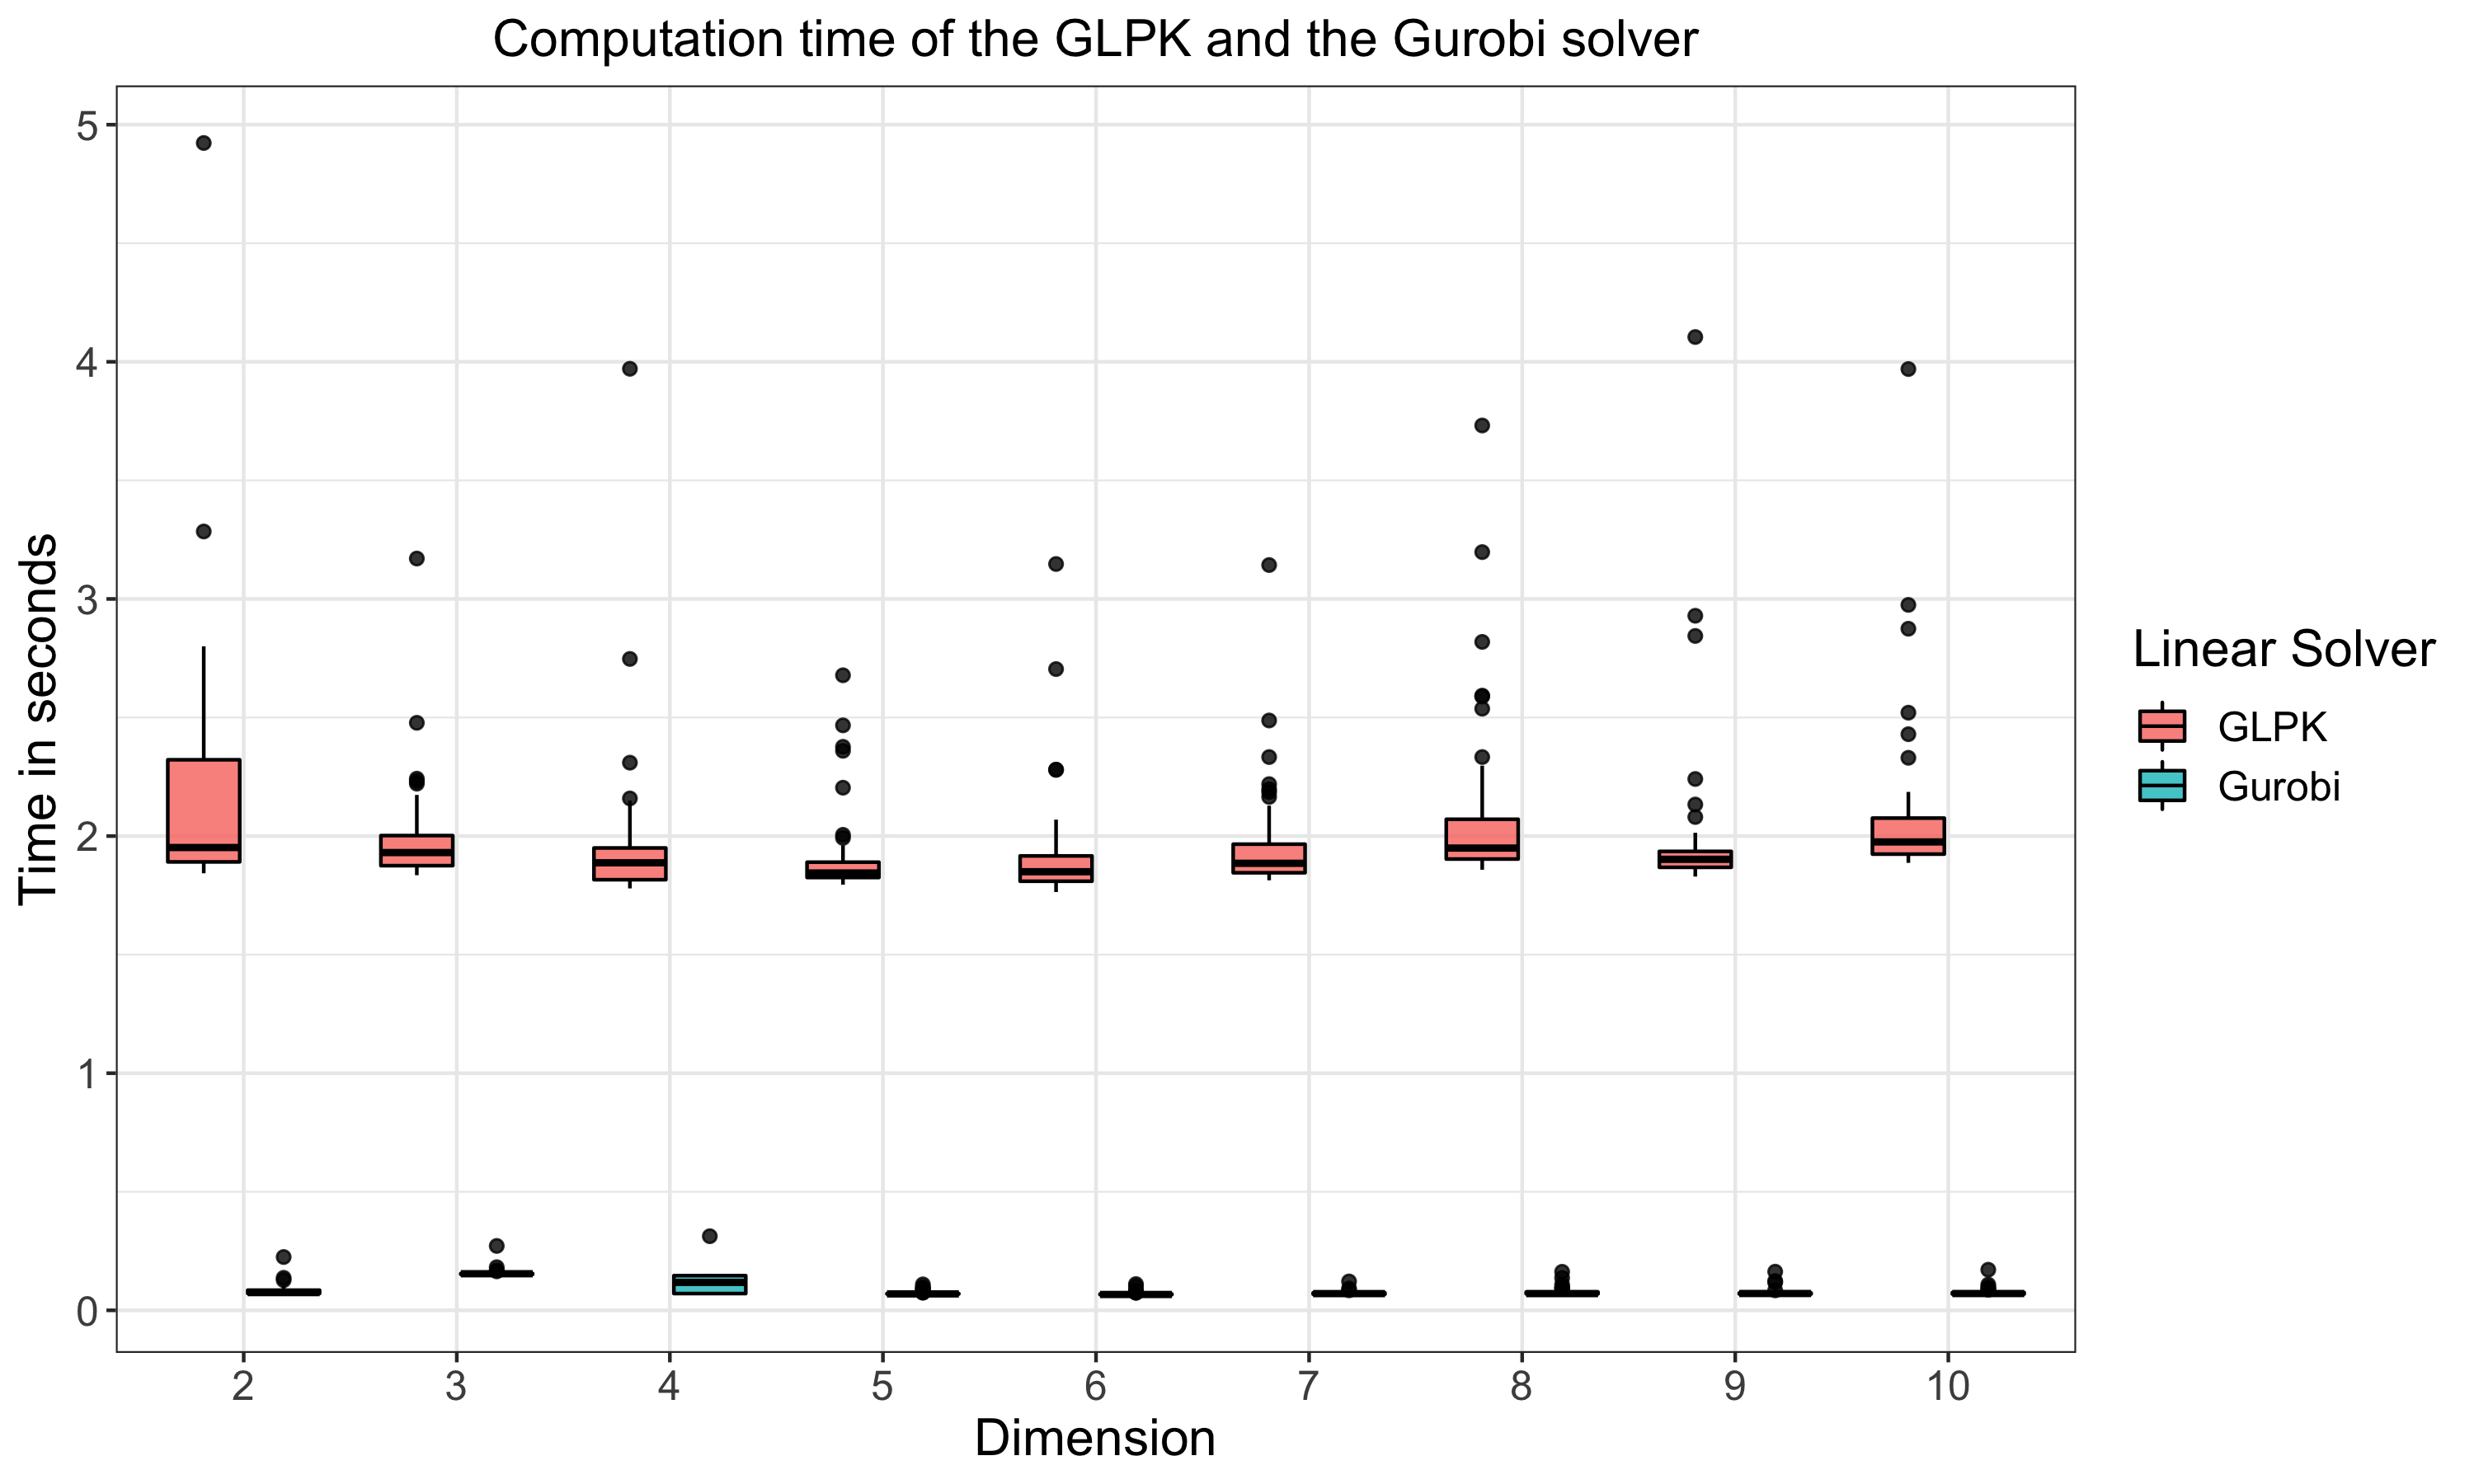
\includegraphics[width=1\textwidth]{boxplots_glpk_gurobi.jpg}% This is a *.eps file
 \end{center}
 \caption{Computation time of the GLPK linear solver (red) and the Gurobi linear solver (green) to solve the uniform/length-weighted edge-loss minimal problems in Algorithm 1. We perform experiments on $90$ data sets, 10 for each dimension 2-10, generated from the normal distribution. The horizontal axis is the dimension of the data set, and the vertical axis is the time it takes to solve an optimization problem. We observe that the Gurobi solver is consistently faster than the GLPK solver and that computation time seems fairly constant across dimension.}\label{fig:glpk_gurobi}
 \end{figure}

% % \begin{figure}[h!]
% % \begin{center}
% % 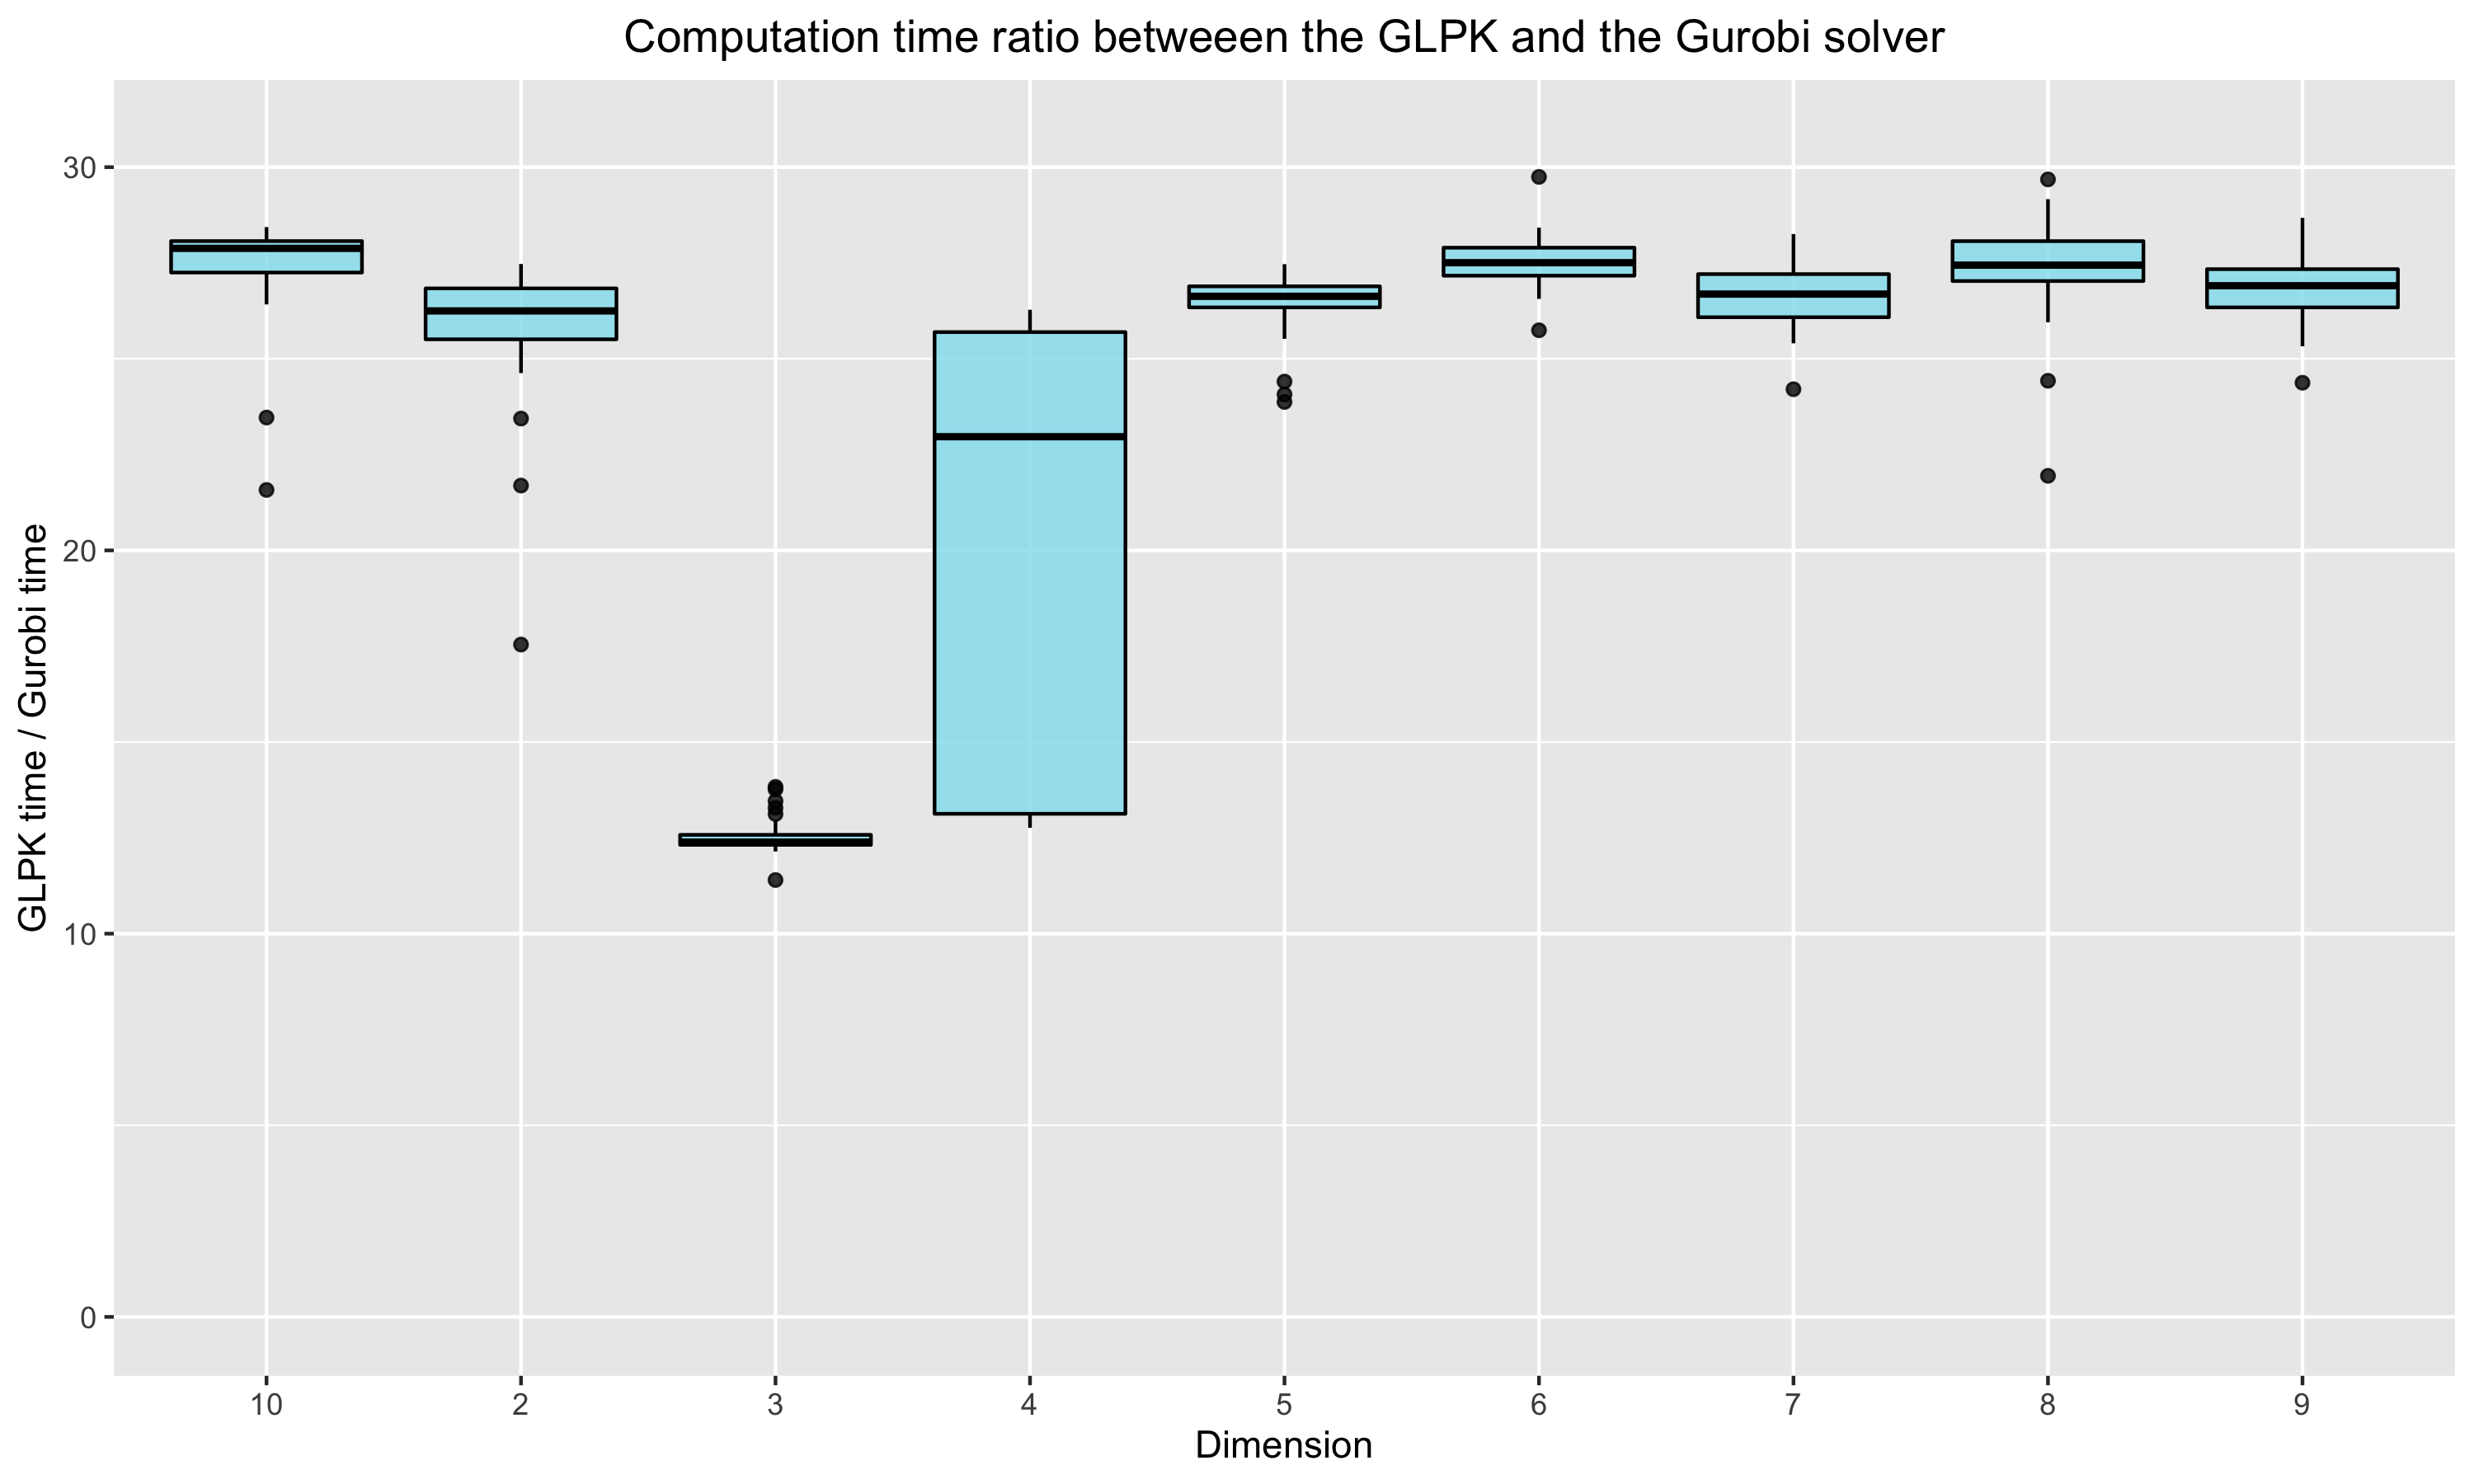
\includegraphics[width=1\textwidth]{figures/computationratio_glpk_gurobi.png}% This is a *.eps file
% % \end{center}
% % \caption{Computation time ratio of the GLPK and Gurobi linear solver. We observe that the Gurobi solver can be a lot faster than the GLPK solver.}\label{fig:glpk_gurobi}
% % \end{figure}


\setlength{\tabcolsep}{9pt}

\renewcommand{\arraystretch}{1.5}
\begin{center}
\begin{table}[]
\caption{{\normalsize{Classifying the coefficients of the optimal cycles for all of the real-world data discussed in Section 5.1 as well as all of the synthetic sets discussed in Section 5.2. The rows are labeled by the coefficient type of the cycle representatives: ``Integral'' means the coefficients for the cycle representative $\optimalrep$ are in $\mathbb{Z}$ and ``In $\{-1,0,1\}$'' means the coefficients for the representative $\optimalrep$ are in $\{-1,0,1\}$. For the columns, $\optimalrep$ represents the optimal representative with its superscript indicating the type of optimization problem: $I$ for integer programming and $NI$ for linear programming, and its subscript indicating the type of optimal cycle: ${E\text{-}Len}, E\text{-}Unif, T\text{-}Unif$ refer to edge loss length-weighted minimal (minimizing total length of $1$-simplices), edge loss uniform (minimizing total number of $1$-simplices), and triangle loss uniform (minimizing the number of $2$-simplices a cycle representative bounds), respectively.}}}
\centering

% \begin{tabular}{|p{2cm} ||p{0.6cm} p{0.6cm} p{0.6cm} p{0.6cm} p{0.6cm}|p{0.6cm}| |p{0.6cm}|p{0.6cm}|p{0.6cm}|p{0.6cm}|p{0.6cm}|p{0.6cm}|}

{\scriptsize{ \begin{tabular}{ |>{\centering}m{7em} *{10}{>{\centering\arraybackslash}m{2.5em} }|}
 \hline
 & \multicolumn{10}{c|}{\textbf{Edge-loss filtered homological optimal cycles} (Program \eqref{eq:edgelossgeneral})} \\
\hline
& \multicolumn{4}{c}{\textbf{Randomly Generated Data Sets}} & & 
 \multicolumn{4}{c}{\textbf{Real-World Data Sets}} &  \\  \cline{2-5}  \cline{7-10}

\textbf{Coefficient Type} & $\x\I_{E\text{-}Len}$ & $\x\NI_{E\text{-}Len}$ & $\x\I_{T\text{-}Unif}$ & $\x\NI_{E\text{-}Unif}$ &  & $\x\I_{E\text{-}Len}$ & $\x\NI_{E\text{-}Len}$ & $\x\I_{E\text{-}Unif}$ & $\x\NI_{E\text{-}Unif}$ & \\
\hline
\textbf{Integral}  & $100\%$ &$100\%$&   $100\%$ & $100\%$ &  & $100\%$ &$100\%$&  $100\%$ & $100\%$ & \\
\textbf{In $\{-1, 0, 1\}$} &  $100\%$  & $100\%$   &$100\%$ & $100\%$ & & $100\%$ &$100\%$&  $100\%$ & $100\%$ & \\ \hline
 & \multicolumn{10}{c|}{\textbf{Edge-loss persistent homological optimal cycles} (\pr (8))}  \\\hline

& \multicolumn{4}{c}{\textbf{Randomly Generated Data Sets}} & & 
 \multicolumn{4}{c}{\textbf{Real-World Data Sets}} &  \\  \cline{2-5}  \cline{7-10}
 \textbf{Coefficient Type} & $\x\I_{E\text{-}Len}$ & $\x\NI_{E\text{-}Len}$ & $\x\I_{T\text{-}Unif}$ & $\x\NI_{E\text{-}Unif}$ &  & $\x\I_{E\text{-}Len}$ & $\x\NI_{E\text{-}Len}$ & $\x\I_{E\text{-}Unif}$ & $\x\NI_{E\text{-}Unif}$ & \\

\hline 
\textbf{Integral}  & $100\%$ &$100\%$&   $100\%$ & $100\%$  &&  $100\%$ & $100\%$ &  $100\%$ & $99.94\%$ & \\
\textbf{In $\{-1, 0, 1\}$} &  $100\%$  & $100\%$   &$100\%$ & $100\%$ &  & $100\%$ & $100\%$&  $100\%$ & $99.94\%$ & \\ \hline

& \multicolumn{10}{c|}{\textbf{Triangle-loss optimal cycles} (\pr \eqref{eq:trianglelossgeneral})}  \\\hline
& \multicolumn{4}{c}{\textbf{Randomly Generated Data Sets}} & & 
 \multicolumn{4}{c}{\textbf{Real-World Data Sets}} &  \\  \cline{2-5}  \cline{7-10}
 \textbf{Coefficient Type} & $\x\I_{T\text{-}Unif}$ &    $\x\NI_{T\text{-}Unif}$ & $\x\I_{T\text{-}Area}$ & $\x\NI_{T\text{-}Area}$  &  & $\x\I_{T\text{-}Unif}$ &    $\x\NI_{T\text{-}Unif}$ & $\x\I_{T\text{-}Area}$ & $\x\NI_{T\text{-}Area}$ &\\
\textbf{Integral}  &  $100\%$ &$99.99\%$ &$100\%$ &$100\%$  &  & $100\%$ &  $100\%$ &  $100\%$ & $100\%$  & \\
\textbf{In $\{-1, 0, 1\}$} &  $100\%$ &$99.99\%$ &$100\%$ &$100\%$  &  & $100\%$ &  $100\%$ &  $100\%$ & $100\%$  & \\ \hline

\end{tabular}
}}
\label{entry}
\end{table}
\label{tab:IntegerCoefficients}
\end{center}


%\bibliographystyle{frontiersinSCNS_ENG_HUMS} %  for Science, Engineering and Humanities and Social Sciences articles, for Humanities and Social Sciences articles please include page numbers in the in-text citations
%\bibliographystyle{frontiersinHLTH&FPHY} % for Health and Physics articles
%\bibliography{test}

\bibliographystyle{formatting_stuff/frontiersinHLTH&FPHY} % for Science, Engineering and Humanities and Social Sciences articles, for Humanities and Social Sciences articles please include page numbers in the in-text citations
%\bibliographystyle{frontiersinHLTH&FPHY} % for Health, Physics and Mathematics articles
\bibliography{test}


\end{document}
